
%%% settings from original file
%\usepackage{geometry}				%No idea what it's good for, but nothing works without it!
%\usepackage{graphicx}				% Use pdf, png, jpg, or eps§ with pdflatex; use eps in DVI mode
%\usepackage{expex}                			%For example formatting
%\usepackage{fontspec,xltxtra,xunicode} 	%These packages help with the fonts
%\usepackage{booktabs}				%This package helps with tables
%\usepackage{fancyhdr}				%This package makes headings look fancy
%\usepackage[table,xcdraw]{xcolor}
%\usepackage{float}					%This package makes tables stay in the right place
%\usepackage[section]{placeins}
%\usepackage{natbib}					%Bibliography package
%\bibliographystyle{anthling}
%\bibpunct[:]{(}{)}{,}{a}{}{;}
%\floatstyle{plaintop}
%\usepackage{caption}					%Package that helps with fussing about captions
%\usepackage{titlesec}
%
%\titleformat
%{\chapter} % command
%[display] % shape
%{\bfseries\Large\itshape} % format
%{Chapter \ \thechapter} % label
%{0.5ex} % sep
%{
%    \rule{\textwidth}{1pt}
%    \vspace{1ex}
%    \centering
%} % before-code
%[
%\vspace{-0.5ex}%
%\rule{\textwidth}{0.3pt}
%] % after-code
%
%\captionsetup[table]{justification=raggedright, singlelinecheck=false, labelfont=bf}
%\geometry{letterpaper}                   		% ... or a4paper or a5paper or ...
%%\geometry{landscape}                		% Activate for for rotated page geometry
%\renewcommand{\baselinestretch}{2}    	%This sets the line spacing
%%!TEX TS-program = xelatex
%%!TEX encoding = UTF-8 Unicode
%\defaultfontfeatures{Mapping=tex-text}
%\setromanfont{Times New Roman}
%\setsansfont[Scale=MatchLowercase]{Arial}
%\setmonofont[Scale=MatchLowercase]{Courier}
%\setcounter{secnumdepth}{5}
%\newfontfamily{\U}{Doulos SIL}
%% TeX will automatically convert eps -→ pdf in pdflatex
%\gathertags % write tags to external tag file
%\Lingset{everygla=\upshape} % make first gloss line upright




\chapter[Losing one's way]{\vspace{-25pt}Losing one's way: Geographical and moral lessons in the Butterfly Story in Upper Tanana Athabascan}

\sethandle{10125/24843}

% \usepackage[
% 	doi=false,
% 	backend=biber,
% 	natbib=true,
% 	style=biblatex-sp-unified,
% 	citestyle=sp-authoryear-comp]{biblatex}
%\usepackage[style=ldc.bst]{biblatex}



% Author last name as it appears in the header
\def\authorlast{Brucks \& Lovick}

% change author in three references below to the actual author name so that this name is unique and matches the \label commands just below and at the end of the chapter
\renewcommand{\beginchapter}{\pageref{brucks-ch-begin}}
\renewcommand{\finishchapter}{\pageref{brucks-ch-end}}
\label{brucks:brucks-ch-begin}



\thispagestyle{firststyle}

\chapauth{Caleb Brucks}
\affiliation{University of Regina}

\chapauth{Olga Lovick}
\affiliation{First Nations University}

\authortoc{Caleb Brucks and Olga Lovick}





\section{Introduction}
\label{brucks:section:introduction}

In this paper, we investigate the use of directional adverbs as indicators of moral confusion in four tellings of the Butterfly story, an important traditional narrative of the Upper Tanana Athabascans of Alaska and the western Yukon. We offer a summary of the story below; the numbers in this summary refer to a story map we created based on conversations with and maps drawn by the storytellers (Figure~\ref{brucks:fig:epmap}).

\begin{figure}[!ht]
    \centering
%    \setlength\fboxsep{0pt}
 %   \setlength\fboxrule{0pt}
    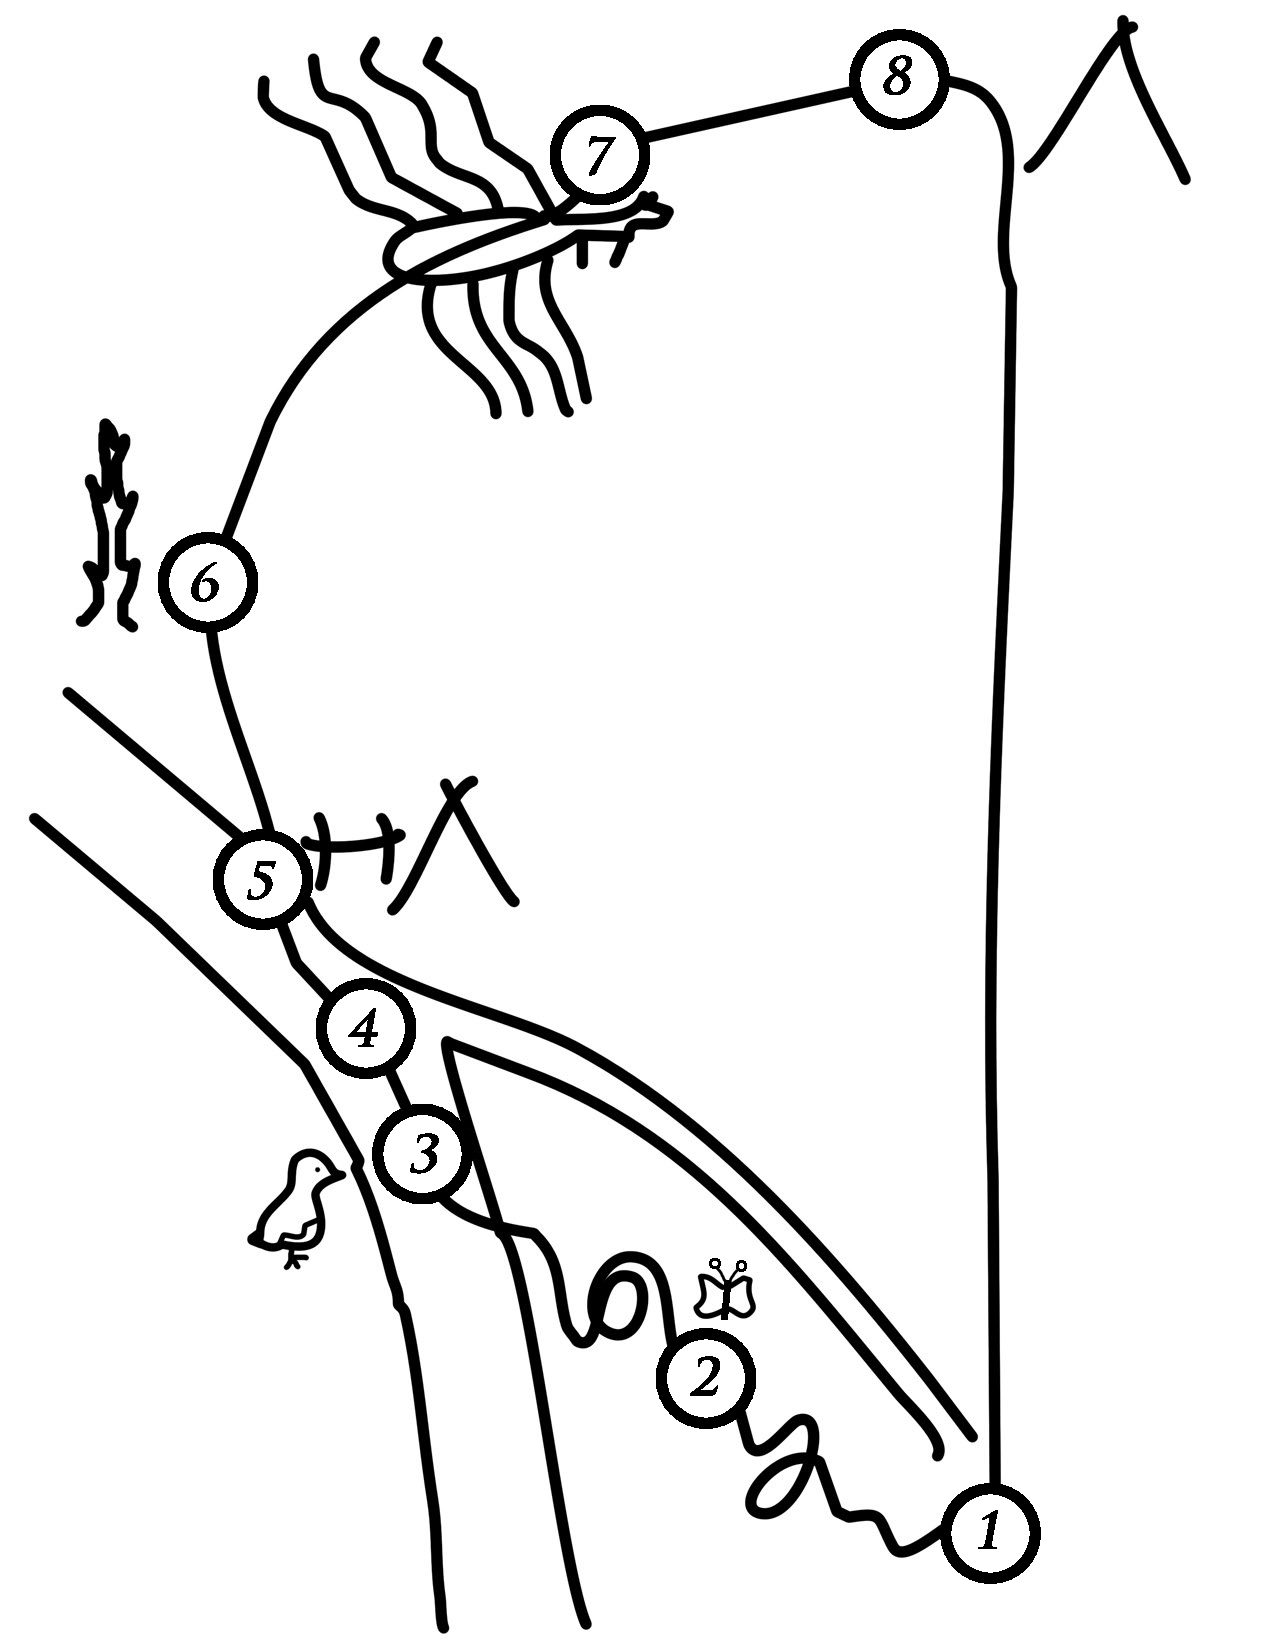
\includegraphics[width=0.7\textwidth]{figures/brucks-fig1} %twogirlsmap
    \caption{Episodes of the Butterfly Story}
    \label{brucks:fig:epmap}
\end{figure}

\begin{quote}
(1) Two Girls follow a Butterfly that leads them astray (2), and they get lost. As they walk upland, they encounter a Chickadee (3) who tells them about a crossroads (4) where they have the choice between two trails. Chickadee advises the Girls to follow the narrow trail, which will lead them home, but does not say what awaits if they follow the wide trail. The Younger Sister wants to take Chickadee's advice, but the Older Sister insists on them taking the wide trail. They then encounter an Old Man (the Devil) living all by himself (5). There are many signs that he is an evil person; for example he has a drying rack with dog skulls on it, or he serves the Girls soup with eyes in it. The Older Sister ignores these warning signs and sleeps with him; she is raped by him with a red-hot iron penis and dies. The Younger Sister remains wakeful through the night and watches her Sister's murder. In the morning, she escapes with the help of a Tree Stump (6) and runs away to a river that she crosses on the tail of a Fox (7). She finally arrives at the tent of an Old Lady (8) who is variously identified as {\em Saa Wunąą} `the Mother of the Sun' or {\em Tsǫǫ Kelahdzeey} `Grandmother Spider'. When the Devil catches up with her there, the Old Lady kills him by melting his flesh with her gaze. The Younger Sister turns his bones and organs into edible plants. She stays with the Old Lady for a while, but is so homesick that she descends through a hole between the worlds to her family, using a rope that she made from moose sinew over a period of many days. When she returns, it begins to snow, a sign that the Old Lady has been killed by her sons.
\end{quote}

In his introduction to Mrs. Mary Tyone's version of this story, James Kari notes that it may be ``regarded as a cautionary tale for young girls'' \citep[23]{TyoneM1996}. Young people are encouraged to follow the `narrow' trail of morality. The Older Sister's insistence on taking the wide trail is punished by rape and death; the Younger Sister only narrowly escapes this fate. (While this piece of advice smacks strongly of Christianity, it is present in all recorded versions of the story, suggesting that it pre-dates missionary influences.) Also important is listening to one's elders; the Older Sister ignores Chickadee's advice and gets killed while the Younger Sister listens and survives. Another lesson is to pay attention, both geographically (to one's surroundings) and morally (to one's behavior).\footnote{\citet[468]{GuedonMF2005} arrives at different lessons contained in this story: ``Ne vous éloignez pas du groupe, ne parlez aux étrangers, faites bien attention à ce qui se passe autour de vous.'' (Don't go away from the group, don't talk to strangers, pay close attention to what happens around you. Translation by the authors.)}

The story follows a circular trajectory, leading the Girls first up and away from their parents into another world, then through a mythological landscape, and finally back down to their parents. The audience is able to follow this trajectory by paying attention to the directional adverbs so pervasive in Northern Athabascan storytelling \citep{KariJ2010, KariJ2011}, which create a `virtual landscape' of the events. As other authors have noted of Athabascan storytelling, directionals, in addition to place names, enable listeners to follow the events of the story ``like a map'' \citep[62]{CruikshankJ1990, MoorePTlenD2007}. This is allowed by the deictic nature of directionals which create a point of view from which to view events which is ``just like being there'' \citep[58]{MooreP2002}. Busch reiterates this view for the Gwich'in saying that listeners can ``form very clear images of the location of actions and the direction of movement being described'' \citet[1]{BuschJ2000}\footnote{For more on the role of directionals in creating narrative space in Upper Tanana stories see \citet{BrucksC2015}.}.

What is striking about this particular narrative is that the Girls lose their way; first in the physical world after following the Butterfly and then in the spiritual world during their encounter with the Old Man. We contrast the serious reduction of directional use in the episodes involving the morally deficient Old Man against the more robust use of directionals—and other spatial descriptions—in the episodes involving the the other (helpful) characters. As we will show in this paper, the storytellers skillfully convey a sense of disorientation—both moral and spatial—by severely curtailing their use of directional adverbs during the episodes involving the Old Man.

The explicit sexual content of the Butterfly story, and in particular the many deviations from what the Upper Tanana consider normal sexuality, is one of the most troubling aspects of this story. Respecting the wishes of several Elders we work with, we will touch on these issues only briefly throughout the paper. We did however make the decision to include them in the discussion, since the deep immorality of the Devil will not otherwise become clear.

This paper is structured as follows. In § \ref{brucks:section:background}, we provide some background information on the Upper Tanana language and on the four versions of the story discussed here. We also give a brief introduction to directional adverbs in Upper Tanana. In § \ref{brucks:section:losing-direction}, we look at what the use of directional adverbs reveals about the Girls' travel through geographic space before turning to the moral disorientation caused by the Devil in § \ref{brucks:section:losing-moral-direction}. We show that the moral disorientation is reflected in the use of directional adverbs and (verbal) prefixes in § \ref{brucks:section:discussion}.

\section{Background}
\label{brucks:section:background}

Upper Tanana is an Athabascan language spoken in eastern interior Alaska and the western Yukon Territory. \citet{MinouraN1994} distinguishes five dialects: Beaver Creek (in the Yukon), Scottie Creek, Northway, Tetlin and Nabesna. Documentation of Upper Tanana was done by SIL linguist Paul Milanowski, resulting in a partial bible translation \citep{MilanowskiPJohnA1966, MilanowskiPJohnA1972} and a Junior Dictionary \citep{MilanowskiPJimersonS1975, MilanowskiPJohnA1979}. James Kari contributed by collecting place names \citep{KariJ1997UTmap}, doing lexicographical work \citep{KariJ1997stem}, and editing a story collection \citep{TyoneM1996}. Several linguistic articles on Upper Tanana can be found in \citet{MinouraN1994, MinouraN1997, TuttleSLovickONunez-OrtizI2011}, and \citet{LovickO2012a-metaphor, LovickO2012b-genre}.

Today, Upper Tanana is severely endangered. There are only 50–90 remaining speakers, and most of them are elderly. There are no more speakers of the Scottie Creek dialect (documented primarily by James Kari) and only a 2–3 speakers of the Nabesna dialect. The Tetlin dialect is also severely endangered with fewer than 10 speakers, while the Northway and Beaver Creek dialects are both still relatively healthy with estimates of more than 20 speakers per dialect.

The observations in this paper are drawn from four tellings of the Butterfly Story. The oldest of these is by the late Mrs. Mary Tyone. It was recorded by James Kari in November 1992; some corrections were made in 1994 before its publication in \citet[23–33]{TyoneM1996}. Mrs. Tyone was a speaker of the Scottie Creek dialect.

The second version was told by the late Mrs. Cora H. David of Tetlin in April 2008 and was recorded by Olga Lovick; it is published in \citet[118–133]{DavidC2011}. Mrs. David was a speaker of the Tetlin dialect.

The third version was told jointly by the late Mrs. Darlene Northway of Northway and Mrs. Jeanie Sanford of Mentasta; it too was recorded by Olga Lovick. The speakers took turns telling the story. Mrs. Northway was a speaker of the Northway dialect; Mrs. Sanford is a speaker of the Beaver Creek dialect.

The fourth version was told by Mr. Roy H. David Sr. (the husband of Mrs. David) of Tetlin in November 2014 and was recorded by Caleb Brucks and Olga Lovick. Mr. David is a speaker of the Tetlin dialect.

Not surprisingly, the two stories told by Mrs. and Mr. David (both from Tetlin) are very similar; Mr. David however explicitly states that he learned this story from (among other people) his mother-in-law—Mrs. David's mother. Similarly, Mrs. Northway's and Sanford's telling is in many places quite similar to Mrs. Tyone's—both of them credited Mrs. Tyone as one of their teachers.

The version by Mrs. Tyone was transcribed and translated by James Kari and Mrs. Tyone; the other versions by Olga Lovick and Caleb Brucks with the help of several speakers of Upper Tanana. While the orthography employed by us follows largely that devised by James Kari as represented in \citet[xi-xvi]{TyoneM1996}, there are some differences. Some of these have to do with dialect; to give an example, the Tetlin dialect does not distinguish the vowels written as <a> and <ä>, so both are represented as <a> in that dialect (see \citealp{TuttleSLovickONunez-OrtizI2011} for more detail); also, in the Northway and Tetlin dialects, the diphtong <įǫ>, which still exists in the eastern dialects, has merged with <ǫǫ> and <iu> with <uu> \citep{LovickO2011}. Other differences may represent variant pronunciations or analyses; for example, Kari writes the vowel of the third person plural object prefix usually long as {\em huu}-, while Lovick tends to write it short as {\em hu}-. For the purposes of the present paper, the spelling of Tyone (1996) is retained in examples taken from that book. The original free translations are also retained here; word glosses have been added by the authors.

The class of adverbs commonly referred to as directionals is a major contributor to spatial description in the Upper Tanana language. Directional forms are made up of three parts: one of nine stems which denote an angle of direction, one of four suffixes (Allative `towards', Ablative `from', Punctual `at a point', Areal `in a general area'), and a prefix of relative distance. The stems and suffixes are synchronically fused so that the stem-suffix combination is now considered a complex stem in Upper Tanana \citep[591]{LeerJ1989}. Prefixes are common but not obligatory. The Proto-Athabascan reconstructions in Table \ref{brucks:table:dir-adv} are taken from \citet[616]{LeerJ1989}.

\begin{table}
\caption{Directional stems in Proto-Athabascan and Upper Tanana}
\label{brucks:table:dir-adv}
\begin{tabular}{ l | l l l l l }
English & Proto-Athabascan & Upper Tanana \\
 & & ALL & ABL & PUNC & AREAL \\ \hline
‘up above’ & *deG & degn’ & dǫǫ {\em or} doo & daa & dogn \\
‘down below’ & *yeG, yex & shyign' & shyǫǫ & shyiit & shyuugn \\
‘upstream’ & *niʔ & ne' & nǫǫ {\em or} noo & noot & nuugn \\
‘downstream’ & *daʔ & da' & dǫǫ {\em or} doo & daat & duugn \\
‘upland’ & *neG & negn' & nǫǫ {\em or} noo & niit & nogn ~ nuugn \\
‘downland’ & *cenʔ & tthän' & tthǫǫ & tthiit & tthuugn \\
‘ahead’ & *nәsd & noo' {\em or} noo & ? & ? & noogn \\
‘across’ & *ŋaˑnʔ & naan' & nǫǫ & naat & nuugn \\
‘away’ & *ʔαnʔ & ’än' & ’ǫǫ & ’aat & ’ogn {\em or} ’oogn \\
\end{tabular}
\end{table}

The Upper Tanana adverbial directional system is anchored to the main waterway of the area. The largest and most important river of the area, the Tanana, begins at the confluence of the Chisana and Nabesna rivers near Northway and runs a little north of west until it flows into the Yukon several hundred miles away. Five of the nine directional stems directly reference the Tanana creating a four-way ``intermediate absolute landmark" system (\citealp[90-91]{LevinsonS2003}, \citealp[129]{KariJ2010}). This subset of the directional adverbs often referred to as `riverine directionals' include the opposing pairs of {\em negn'} `upland' vs. {\em tthän'} `downland',  {\em ne'} `upriver' vs. {\em da'} `downriver', and {\em naan'} `across', which is its own opposite \citep[576]{LeerJ1989}. They match the general east to west flow of the river but are also largely abstracted. As such, the directionals can be used when well away from the Tanana river if still in the same region. For example,  {\em negn'} `upland' can be used when travelling upstream on the Nabesna as it is `upland' viewed from the Tanana.

In addition to the regional uses of the riverine directionals, directionals can be used in local settings to refer to the upriver direction of a minor tributary or to point across local landmarks such as lakes or treeless flats. The remaining (non-riverine) directionals are generally used in this local manner as well. {\em Degn'} `up (vertically)' and {\em shyign'} `down (vertically)' are used in settings like `up (a tree)' and or `down (on the floor)' as well as `uphill' or `downhill' with no (horizontal) direction specified. The remaining stems are vague in their directional content. The `ahead' {\em noo'} stem does not specify any set direction though it is often used when moving out in to open areas and {\em 'än} is even more devoid of spatial content with a general `away, outside' meaning. The directional stems are also extended to a number of other settings—such as the interior of houses (see \citealp[131]{KariJ2010} for more examples). While the use of directionals likely have a historical origin in the normal orientation of houses to the river (see \citealp{FortescueM2011} and \citealp[602]{LeerJ1989}), the directional stems in Upper Tanana are removed from their direction-bearing content and lexicalized as discrete forms, such as {\em ne'} `side of the house' or `rear, behind (gun, animal, person, etc.)' for instance. A clear example of this is found with the {\em 'än} `away' stem which takes the meaning `outside (the house)' and is the opposite of {\em noo'} `inside, toward the center (historically: the fire)'. In these cases, then, the directional stems are more than ample to describe the `microcosm' \citep[7]{FortescueM2011} inside the house but are of a different type from the directionals used in reference to rivers or major landmarks.

Upper Tanana also has a rich inventory of adverbial verb prefixes. These are part of what \citet[28]{KariJ1979} terms `aspectual derivational strings', which are discontinuous morphemes with clear semantic content (e.g. {\em ske}- `across a body of water' or {\em dzi-na}- `down over an edge') that apply productively to a number of verbs. A substantial subset of these prefix strings is used to describe motion through space, and derives a number of motion verbs. While our focus in this paper lies on the use of directional adverbs, we will occasionally make reference to directional prefix strings where they serve to clarify the motion described in the narrative.

\section{Losing one's place}
\label{brucks:section:losing-direction}

The story begins with the Two Girls chasing a Butterfly. They then become lost and at some point leave `our' world behind and enter a world on top of the sky. It is intriguing, though, that the versions differ in when exactly this transition between worlds takes place. In Mrs. Tyone's version, the transition happens at the very beginning of the story as demonstrated in (\ref{brucks:tyone-transition-to}).\footnote{The following abbreviations are used in this paper: CT—contrastive topic, \textsc{foc}—focus, PL—plural.}

\begin{exe}
\ex Transition into the world above the sky (Mrs. Tyone) \label{brucks:tyone-transition-to}
\begin{xlist}

\ex \gll Dziin uudih Laalil nahnetdik.  \\
 day all butterfly {they kept following around} \\
\glt `All day long they followed butterflies.' \\

\ex \gll Ishyiyit t'eey t'axo Laalil huu'eh keenän'ii'ąą.  \\
 then even finally butterfly {with them} {it took the world up} \\
\glt `And then, all of a sudden, Butterfly took them up to another world.' \\

\ex \gll Yaat'agn tah huu'eh nän' ninii'ąą.  \\
 {through sky} among with them earth {it took up} \\
\glt `It took them through the sky into another world.'  \\

\ex \gll Ishyit tąy haadäl eh huu' nduu {huu'eh huushyaak} ts'ą̈'.  \\
 there trail {they were going} and ? somewhere {they got lost} and \\
\glt `They were going on the trail there, and they got lost somewhere.' \\
\end{xlist}
\end{exe}

In the version by Mrs. David, given in (\ref{brucks:davidc-transition-to}), the Girls cross into another world very early as well. Note that in (\ref{brucks:davidc-transition-to}a-b), the Girls' mother explicitly warns them not to follow the Butterfly.

\begin{exe}
\ex Transition into the world above the sky (Mrs. David) \label{brucks:davidc-transition-to}
\begin{xlist}

\ex \gll Hunąą huts'ą' ehsał nts'ą': ``Ena'! Sǫ'!''  \\
 {their mother} {to them} hollered and no don't \\
\glt `Their mother hollered at them: ``No! Don't!'' ' \\

\ex \gll ``Laalil natnatdagn stanuhtaałeeł nt'eh,'' hu'ehnih.  \\
 butterfly {you, following} {he will take you away} certainly {she told them} \\
\glt ` ``If you follow the Butterfly, he'll take you away for sure,'' she said to them.' \\

\ex \gll T'oot'eey k'at'eey hiidiitth'agn nts'ą' Laalil \textbf{nahdogn} ch'idanh keey k'it tah kehu'įįdlah.  \\
 but not {they didn't listen to her} and butterfly up different village on among {it took them} \\
\glt `But they did not listen to her, and the Butterfly took them up to a different world.' \\

\ex \gll Eł hu'ihuushyaak.  \\
 and {they got lost} \\
\glt `And they got lost.' \\
\end{xlist}
\end{exe}

In both versions, following the Butterfly is the direct cause of the Girls' getting lost. In (\ref{brucks:tyone-transition-to}), the Butterfly takes the earth, {\em nän'}, as a single round object through the sky; the Girls are taken together with the earth. In Mrs. David's version, the Butterfly takes a plural object—the Girls—up into a different `village': a different world. The notion of `up' in (\ref{brucks:davidc-transition-to}) is expressed in several ways: by the directional adverb {\em nahdogn} `Area above', by the postposition {\em k'it} `on top', and finally by the prefix string {\em ke}- `up, against' in the verb form {\em kehu'įįdlah} `it took them', which also occurs in themes describing other types of vertical motion, e.g. climbing a tree.

In the version told by Mrs. Northway and Mrs. Sanford, the Girls simply get lost; the narrators do not explicitly state at which point the transition into the other world takes place. In the version told by Mr. David, crossing into the world above the sky seems to happen in stages. The Butterfly leads the Girls away in the uphill direction where they get lost.

\begin{exe}
\ex Transition into the world above the sky (Mr. David)\label{brucks:davidr-transition-to}
\begin{xlist}

\ex \gll Hǫǫ tay' hidetnii huch'a tah niłk'ineht'ah niłk'ineht'ah huch'a.  \\
 thus again {they grabbed it} {from them} among {it fluttered around} {it fluttered around} {from them} \\
\glt `Again they tried to grab it but it fluttered away from them, it fluttered away from them.' \\

\ex \gll Niłk'ineht'ah huch'a nahiitnetdak  \\
 {it fluttered around} {from them} {they started following it}\\
\glt `It fluttered away from them and they started following it.' \\

\gll Tąy nts'ą' t'eey stahuunįįdlah, \textbf{deg'} uudih. \\
 trail to even {he took them away} {up vertically} {totally} \\
\glt `He took them away to a trail, all the way up.' \\

\ex \gll Ddhał taag ch'ale',  ddhał taag tah, \textbf{deg'} tah, \textbf{deg'} tah hu'aałeeł ndee hiits'ihetniign.  \\
 mountain three \textsc{foc} mountain three among {up vertically} among {up vertically} among {it was taking them} {where to} {they didn't know}  \\
\glt `Over three mountains, over three mountains, up and up it took them, they did not know where to.'\\
\end{xlist}
\end{exe}

In subsequent conversations, Mr. David clarified that while the Girls have left `our' world behind in crossing the mountains, they have not yet entered the world above the sky. The Younger Sister arrives in the place above the sky only after she has crossed the river with the help of Fox. At that point of the story, the Older Sister has been killed and the Younger Sister is running from the Devil. If we understand Mr. David correctly, then the Girls' journey to another world is very gradual; they leave their own world while chasing the Butterfly, but their crossing between worlds is incomplete until the Younger Sister comes to the river (Authors' fieldnotes, November 20, 2014).

At first glance, it is surprising that the narrators disagree about the exact place of the crossing. But as \citet[470f.]{GuedonMF2005} convincingly shows, the boundaries between the two worlds are not fixed in Upper Tanana cosmology: any place can serve as entry point, and many animals can serve as guides from one world into the other. Moreover, the landscape of the world above the sky so closely resembles ours—with hills, trees, flats, and rivers—that it is not surprising that at first, the Girls do not notice that they have come to a different place, with different rules and different dangers. Here as well as elsewhere, though, there are ``good'' and ``bad'' roads to travel (cf. \citet[473]{GuedonMF2005}, and the Girls will have to figure out which is which.

Soon after getting lost, the Two Girls reach a crossroads. A Chickadee advises the Girls to take the narrow trail and explicitly warns them off the wide one. This passage, as told by Mrs. David, is given in (\ref{brucks:cora-chick}); the versions by Mrs. Tyone and Mr. David are very similar to this. In the version told by Mrs. Northway and Mrs. Sanford, the Girls have to decide on their way without Chickadee's help.

\begin{exe}
\ex Chickadee's advice (Mrs. David) \label{brucks:cora-chick}
\gll {Ay eł} Ts'igąąk: ``Tąy ts'eegn k'e ahdeeł, sǫ' tąy teeł k'e ahdeel,'' hu'ehnih. \\
 and Chickadee trail narrow on {you go} don't trail side on {you don't go} {he told them} \\
\glt `And Chickadee said to them: ``Go on the narrow trail, don't go on the wide trail!'' \\
\end{exe}

In all versions, the Younger Sister wants to go onto the narrow trail (which would have led them back home), but the Older Sister fights her physically and drags her onto the wide trail (\ref{brucks:decision-dn-js}):

\begin{exe}
\ex Making the decision (Mrs. Northway and Sanford) \label{brucks:decision-dn-js}
\begin{xlist}

\ex \gll Didia' tthiits'äl' uuniik tl'aan \textbf{nahdegn'} tah ch'itsąą tąy \textbf{degn'} tah didia' ditthiixa' eh aałiu.  \\
 {her younger sister} hair {she grabbed} and {up vertically} among different trail {up vertically} among {her younger sister} {her hair} with {she dragged} \\
\glt `She grabbed her Younger Sister's hair and up there onto the other trail she dragged her Younger Sister by her hair.' \\

\ex \gll Ay tl'aan \textbf{hohdegn'} hihteedeel eh \textbf{nah'ogn} łįį tthi' dineh tthi' eetah dahdzäl k'it da'eedlay huunehttheh.  \\
 and then {up vertically} {they started} and {out there} dog skulls man skulls {among them} {drying rack} on {they were up} {they were barking} \\
\glt `And then they began to walk uphill and out there there were dog skulls and human skulls up on the drying rack and they were barking.'   \\
\end{xlist}
\end{exe}

Even though the Girls have left our world behind, the use of directionals continues up to the point where they arrive at the Old Man's camp. Despite having chosen the bad trail, they have retained enough of their sense of orientation to keep going. But the barking skulls on the drying rack are the first indication that something is very, very wrong. As it turns out, the Girls now are not just lost spatially, but they are also in a place where their moral sense of direction will be severely challenged.

\section{Losing one's moral sense of direction}
\label{brucks:section:losing-moral-direction}

The episode where the Two Girls first encounter the Devil is deeply disturbing. The Girls have entered a place where unnatural and immoral activities take place, which challenges their ability to distinguish right from wrong. This episode diverges from the previous sections by introducing the antagonist of the narrative, the Old Man or Devil, who is a morally disorienting force. He encourages the Girls to commit morally questionable acts and seeks to keep the Girls from finding their way home---essentially he aims to keep them ``lost''.

The encounter begins with the Two Girls first meeting with the Devil. In three of the four narratives (Mrs. David's story excluded) the Girls' arrival at his camp is greeted by the barking of dogs. However, the Girls quickly learn that the barking is coming not from dogs but from their parts left on a drying rack.

Mrs. Sanford and Northway's version is the only one where the dogs (their skulls) share the drying rack with human remains (see (\ref{brucks:decision-dn-js}f) above). No less odd, however, are the barking split carcasses of dogs in Mrs. Tyone's story (\ref{brucks:tyone-barking-dogs}) or the barking eyes in Mr. David's version (\ref{brucks:rdavid-barking-dogs}e).

\begin{exe}
\ex Coming in to the Devil's camp (Mrs. Tyone) \label{brucks:tyone-barking-dogs}
\begin{xlist}

\ex \gll \textbf{Xahdogn'} dahdzäł k'it łįį elk'aagn naat da'eedlay.   \\
 {up above} {drying rack} on dog split across {they lie}  \\
\glt `Up above on the rack were split dog carcasses.' \\

\ex \gll  Ay łįį elk'aagn gąy in t'eey ttheehihdelxoh ay'eh ishyiit.  \\
  and dog split dry PL even {they are barking} and there \\
\glt `And those dry dog carcasses were barking right there' \\
\end{xlist}
\end{exe}

\begin{exe}
\ex Coming in to the Devil's camp (Mr. David) \label{brucks:rdavid-barking-dogs}
\begin{xlist}

\ex \gll ``{Dii xa} ndee ts'anh ch'ale łįį needehtthay?''   \\
 why where from \textsc{foc} dog {barking at us}  \\
\glt ` ``Why, where are the dogs barking at us?'' ' \\

\ex \gll ``K'at'eey łįį nak'ąy,'' nih.  \\
 not dogs {I don't see} {she said}  \\
\glt ` ``I don't see any dogs,'' she said.' \\

\ex \gll  \textbf{Nahdegn'} dahdzal k'it uneh'ąy eh tah tth'an' uuł.  \\
  {up vertically} {drying rack} on {she looked} and among bone skeleton \\
\glt `She looked up at the drying rack and [there were] bones, skeletons.' \\

\ex \gll  Ay ch'a Ts'ant'ay łįį atnag.   \\
  and \textsc{foc} Devil dog {he eats} \\
\glt `And this was the Devil, he eats dogs.' \\

\ex \gll  Ay ch'ale unaag' ch'ale hunehtthay.  \\
  And \textsc{foc} {their eyes} \textsc{foc} {barking at them} \\
\glt `And it was their eyes barking at them.' \\
\end{xlist}
\end{exe}

Barking pieces of dead dogs is certainly an odd event and thus strongly signal that the Girls have entered an entirely different world. Importantly, it is also an indication of the immorality of the Old Man. Eating dogs is strictly taboo in the Upper Tanana area as it is among other Athabascan groups. \citet[162]{McKennanR1959} states that the ``Upper Tanana hold the dog in peculiar reverence, and they will neither kill nor eat it although they have no rationalized explanation for this taboo''. \citet{NelsonR1983}, in his discussion of Koyukon relationships with animals, emphasizes the usefulness of dogs as pack and guard animals, but finds their role as companions the most important; dogs have a privileged relationship with humans as their only domesticated animal. Thus, though killing dogs is not taboo when they have outlived their usefulness, eating them definitely is, and \citet[191]{NelsonR1983} suggests that this is because it ``is perhaps akin to cannibalism, given their closeness to humans''. This closeness is clear in that dog owners are referred to as their dog's {\em bitsiya} `grandfather' and that dogs are the only animal to share the plural morpheme {\em -kka} with humans. Though the Upper Tanana neither refer to dogs as their grandchildren or share a human plural with dogs (although dogs are more commonly pluralized than other animals) they share a close relationship with dogs unequaled by any other animal (even today the dog is the only animal kept as a pet) and thus the repulsion to eating them remains strong.

The reverence for dogs is mixed with a certain level of unease with their spiritual power. For example, Koyukon people traditionally did not allow dogs to live in the house as it would make the children behave like dogs which presumably ``means eating unclean things, acting wild and unruly, being half animal'' \citep[191]{NelsonR1983}. A similar fear of the ``unclean'' spirit of dogs is seen in the Upper Tanana taboos which restrict dogs from eating the heads of large game or carcasses of fur bearing animals as it will remove the hunter's or trapper's luck \citep[168]{McKennanR1959}. Similarly, if dogs find the placenta of a newborn child the woman will bear no more children \citep[167]{McKennanR1959}. Dogs are both creatures close to humans as well as unclean and dangerous to them and thus the Devil is committing a doubly abhorrent act by eating them.

However, eating dogs also shows that the Old Man is a different type of being than the Girls—a type of being which finds eating dogs (and humans perhaps) as normal as eating white fish or moose is for the Upper Tanana. That is, this event illustrates the perspectival \citep{ViveirosDeCastroE1998} outlook common in the cosmology and narratives of Alaskan Athabaskans. (While the argument for a perspectival view was originally put forward by Viveiros de Castro based on Amazonian groups, similar arguments have been made for North American groups by \citet{IngoldT2000} for the Ojibwa and \citet{NadasdyP2003} for the Kluane.) In the current narrative, then, the fact that the Old Man eats dogs, something that real people would never do, shows that he is a different type of being: a type of being who sees killing, drying, and eating dogs the same way humans see doing this to moose or caribou.

The version told by Mrs. David does not have barking dog parts at the beginning of the two Girls' encounter with the Devil. Instead, the eating of dogs enters the narrative in a much more direct manner: the Old Man serves the Two Girls a soup with dog eyes in it.

\begin{exe}
\ex Eating dog eyes (Mrs. David) \label{brucks:cdavid-dogs-eyes}
\begin{xlist}

\ex \gll Ch'idia' hashyiign tuuthał shyiit huneh'ąy eł łiign naagn' dii naagn' le' ushyiit natatdiiłek.   \\
 {younger sister} down soup in {she looked} and dog eyes what eyes UNCERT {in it} {were floating} \\
\glt `The Younger Sister looked down into the soup and dogs' eyes and I don't know what sort of eyes were floating in it. ' \\

\ex \gll Eł: ``K'at'eey tih'aal!'' yuunih nts'ą' dushyiign t'eey naatehtl'iit dą' ch'itay nahtak.  \\
 and not {I won't eat it} {she thought} and down even {she spilled} when {old man} {looked away}  \\
\glt `And, ``I'm not going to eat it!'' she thought and she spilled it when the Old Man wasn't looking.' \\

\ex \gll  Ch'aadeh du' naye'aał.  \\
 {older sister} CT {ate it} \\
\glt `The Older Sister however ate it.' \\
\end{xlist}
\end{exe}

Eating the dogs' eyes is problematic in a number of ways. Eyes in themselves are dangerous and children should never touch them as it will cause ``nightmares, cramps, or something worse'' \citep[177]{GuedonM1974}. Also, by ingesting certain foods, one acquires some of the properties of this food, both positive and negative \citep[233]{NelsonR1983}. Young girls who just had their first period may not eat ripe berries, as that is believed to cause excessive bleeding \citep[21]{TyoneM1996}. Young children may not eat moose meat because young moose are so awkward; instead, children are fed caribou meat since caribou are up on their feet just minutes after their birth \citep{DavidCforthc}. Through her action, the Older Sister acquires one of the most salient trait of dogs: inattentiveness \citep[104, 110]{LovickO2012a-metaphor}. Lovick cites the expression {\em Łįį k'eh uht'iin ahłįį} `You guys are like dog people', which according to Mrs. David was used frequently by her own mother when admonishing her children to pay attention and listen to her Elders. Dog people, apparently, do not pay attention and do not listen to advice. By eating dog, the Older Sister becomes more dog-like, less human.

This has disastrous consequences for the Older Sister. She loses her ability to see the world the way a human does it, and thus to distinguish right from wrong; she now views the world in the immoral way of the Devil. She next declares her intention to sleep with the Devil, who recognizes her as an easy victim and kills her by raping her with a red-hot iron pole. The Younger Sister, who has surreptitiously refused to partake of the dogs' eyes, retains her ability to see clearly, and thus escapes the Devil. She has retained her sense of self as a human being (see also \citealp[470]{GuedonMF2005}).\footnote{This interpretation of the significance of eating eyes was confirmed in a conversation with Mrs. and Mr. David on May 17, 2013.}

The episode where the Devil rapes and kills the Older Sister abounds in all variants with verb themes having to do with seeing. In a stretch of text between 4 (Mrs. David) and 25 (Mr. David) lines long, a total of nineteen `seeing' verbs belonging to seven different verb themes is used. This emphasis on seeing stresses the watchfulness of the Younger Sister, especially as compared to the inattentiveness of the Older Sister. Even more importantly, reliance on the sense of sight distinguishes humans from many other animals that rely more on their sense of sound or smell. The Old Man in this story is different, non-human, in that he uses his sense of smell to track down the Girl, just like a dog would do. (The Upper Tanana used dogs frequently as hunting companions and were thus certainly aware of that animal's keen sense of smell.) Crucially, the Devil's following the Younger Sister's scent trail is a feature of all four variants of this story.

At this point of the story, the Older Sister has made several crucial mistakes. She has left home—and presumably her chores—behind to chase after a Butterfly, and she has taken the wrong turn at the crossroads. At the Old Man's camp, she ignores all the warning signs. In both Mr. and Mrs. David's versions, the Old Man is identified as a bad and lying individual from the outset, who pretends to follow Athabascan protocol of welcoming unexpected guests, feeding them and offering a safe place to stay \citep[140]{GuedonM1974}. But the food he offers is unclean, and the place he offers is anything but safe. In these two versions, the Older Sister's lack of judgment manifests itself through the—ordinarily innocuous—act of falling asleep. By abandoning her vigilance, she eventually causes her own death.

In the versions told by Mrs. Tyone and by Mrs. Northway and Sanford, the Old Man does not live entirely alone; opposite him, an Old Lady is staying (in the version told by Mrs. Northway and Mrs. Sanford, this Old Lady is identified as {\em Tsǫǫ Kelahdzeey} `Grandmother Spider'; in Mrs. Tyone's version, the Old Lady remains unnamed). In this version, the Older Sister's loss of moral direction is quite a bit more blatant:

\begin{exe}
\ex Spending the night (Mrs. Northway and Mrs. Sanford) (UTOLAF10Jul0202) \label{brucks:sleep-with}
\begin{xlist}

\ex \gll Ay tl'aan {ts'exeh gaay} ishyiit du' Tsǫǫ K'elahdzeey xa nihnįįdeel eh.  \\
 and then Girl there CT Grandmother Spider for {they arrived} and \\
\glt `And then the Girls went to Grandmother Spider.' \\

\ex \gll Ch'idia' du: ``Stsǫǫ eh tihteeł!''  \\
 {younger sister} CT {my grandmother} with {I will sleep} \\
\glt `The Younger Sister [said]: ``I will sleep with my grandmother!'' ' \\

\ex \gll Ch'aadeh du': ``Stsay eh tatihteeł!''  \\
 {older sister} CT {my grandfather} with {I will sleep} \\
\glt `The Older Sister [said]: ``I will sleep with my grandfather!'' ' \\

\ex \gll Maa hǫǫsǫǫ ditsay eh teete'.  \\
 {for her} good {her own grandfather} with {she will sleep} \\
\glt `She is happy that she is about to sleep with her own grandfather.' \\
\end{xlist}
\end{exe}

By making the decision to spend the night with the Old Man rather than the Old Lady, the Older Sister commits a severe violation of proper behavior. In Upper Tanana culture, young girls are sequestered at the onset of puberty. There are many restrictions regulating their behavior during this period of sequestration as well as afterwards; these (as well as similar rules affecting males) are usually called {\em įįjih} which is variably translated as `forbidden' or `taboo'. Discussions of the many rules affecting young girls can be found in \citet{TyoneM1996} and \citet{DavidCforthc}. Some of these rules regulate the relationships between genders. Generally, girls are supposed to stay away from men because their presence may adversely affect the men's hunting luck; this serves at the same time to prevent sexual promiscuity, which is frowned upon \citep[174, 187, 190]{GuedonM1974}. Chosing to sleep with\footnote{It is not clear whether the Upper Tanana expression for `sleep with' has the same sexual connotations as the English one, but it should be noted that a related verb theme in Koyukon does (see \citealp[496]{JetteJJonesE2000} {\em yʉgh naaltaanh} `he lay down with her, he slept, had sex, copulated with her', and following discussion by Jetté).}  the Old Man rather than the Old Lady, is a severe violation of {\em įįjih}.

In the following episode of the narrative, the Older Sister reaps the consequences of this violation. (This part is identical in all versions of the story.) While she is sleeping, the Devil anally rapes and ultimately kills her using a metal pole that he has heated up in the fire.

The Younger Sister on the other hand retains her moral compass. When the Old Man wants her to defecate on his hands and on his head she wisely refuses, insisting instead on going outside to do this, which also provides her with the opportunity to escape.

\section{Directionals: creating space, creating confusion}
\label{brucks:section:directionals-space-creation}

In this section, we look at how directionals are used at crucial moments in the story. We show that they are used to spatially and morally ground the Girls, and, in three of the versions we look at, also to reflect the Younger Sister's ability to keep her bearings. At the same time, we find that the very absence of directionals is just as meaningful, in that it serves to disorient the audience, thus reflecting the Girl's being lost. As well, the periods of use and non-use of directionals closely match other explicit and implied moral claims about the character of the people the Girls meet.

In all versions of the story the helpful characters (Chickadee, the Tree Stump, Fox, Grandmother Spider) help the Sisters escape their plight by providing direction. Often this includes the use of directional adverbs which serve to place the Girls on the landscape and give them guidance. This directly contrasts with the behavior of the Old Man who refuses to give any sort of direction. A representative example of the direction given by the helpful characters is provided by the Chickadee, who advises the Two Girls to follow the narrow trail. (\ref{brucks:rd-trail}) contains this passage in the version by Mr. David.

\begin{exe}
\ex Chickadee's advice (Mr. David) \label{brucks:rd-trail}
\begin{xlist}
\ex \gll ``\textbf{Ahda'} \textbf{du'ǫǫ} tąy įhhaal shnah'įį?''  \\
 upriver {from out there} trail {I walking} {you saw me} \\
\glt ` ``Up there, from out there, the trail I was walking on, did you see me?'' [Chickadee said]' \\

\ex \gll ``Ąą','' hiiyehnih'.  \\
 yes {they said to him} \\
\glt ` ``Yes,'' they said to him.' \\

\ex \gll ``{Ay nts'ą'} ahdał uchįį ninahdeeł de' tąy łaakay.''  \\
 and {you're going} {its tip} {you arrive} when trail two \\
\glt ` ``And keep going and when you arrive at that point [there are] two trails.'' \\

\ex \gll ``\textbf{Shyiig'} nts'ą' tąy teeł, \textbf{adeg'} du' tąy gaay.''  \\
 {down vertically} toward trail wide {up vertically} CT trail small \\
\glt ` ``Down there is a wide trail, but up there is a small trail.'' ' \\

\ex \gll {Ay ch'a} nahdal tąy gaay, sǫ' tik'i'ahdeel jah tąy nįįteel!  \\
 and {you go} trail small don't {you turn off} here trail wide \\
\glt ` ``And go on the small trail, don't turn off onto the wide trail!'' \\

\ex \gll ``{Neenaattheh dą'} ts'anh \textbf{hutthan'} k'a hihtetdag hǫǫ niłhidetniik,'' nih.  \\
 {long before us} from waterwards not {they don't go} thus {they tell each other} {he said} \\
\glt ` ``From long before us they don't go down there, they tell each other,'' he said to them. \\

\ex \gll ``Tsin'įį,'' hiiyehnih.  \\
 {thank you} {they told him} \\
\glt ` ``Thank you,'' they said to him.' \\

\ex \gll Ts'įįgąąk tay' t'eey ``Sǫ', sǫ' tąy nteel sǫ' \textbf{dahtthän'} tahdeel!''  \\
 Chickadee again even don't don't trail wide don't waterwards {you will not go} \\
\glt `Chickadee again, ``Don't, don't go toward the water on the wide trail!'' \\

\ex \gll ``\textbf{Deg'} ay ch'a nuhnąą iin nuhta' nuhkeey natatdal,'' hu'ehnih.  \\
 {up vertically} and \textsc{foc} {your mother} PL {your father} {your village} {you will return} {he told them} \\
\glt ` ``Up, and you will return to your mother and father and your village,'' he told them.' \\
\end{xlist}
\end{exe}

Chickadee, in his attempt to guide the Girls back onto the right way, gives very precise directions that include not only a description of the trails involved but seven directionals. He also utters an explicit warning against the wide, downland trail (\ref{brucks:rd-trail}h) and promises that they will return if they follow the narrow, uphill trail (\ref{brucks:rd-trail}i).

This explicitness contrasts sharply with the behavior of the Old Man. In none of the versions does the Old Man use a directional to tell the Girls where they are or where they need to go. In the version by Mr. David, the Old Man promises to take the Girls home. But even in this version, given in (\ref{brucks:david-return}), he does not use directionals.

\begin{exe}
\ex No directionals in promise (Mr. David) \label{brucks:david-return}
\begin{xlist}

\ex \gll ``Tsay, shaadeh ts'i'oktiin!''  \\
 grandpa {my older sister} {I want to wake up} \\
\glt ` ``Grandpa, I want to wake my Older Sister!'' [the Younger Sister said.]' \\

\ex \gll ``Ena'! Ena'! Uute'! {Kahman' de' tah} keey nanuhtagshyeeł,'' u'iichijelnih.  \\
 no no {she should sleep} {in the morning} village {I will bring you back} {he lied to her} \\
\glt ` ``No! No! Let her sleep! In the morning I will bring you guys back to the village,'' he lied to her.' \\
\end{xlist}
\end{exe}

The Old Man uses directionals with non-local reference only when talking to himself after the Girl has escaped, for example in (\ref{brucks:northway-talk-to-stump}):

\begin{exe}
\ex Looking for the Girl (Mrs. Northway and Mrs. Sanford) \label{brucks:northway-talk-to-stump}
\gll Ay eh du' ch'itay, ``Nts'ąą' ch'a ts'exeh \textbf{daatthǫǫ} sts'ą̈' hǫǫheey,'' hii'itniik. \\
 and also CT {old man} how \textsc{foc} girl {to downland} {to me} {she speaking} {he thought}\\
\glt `And that Old Man wondered ``How come that Girl is talking to me from down there?'' ' \\
\end{exe}

Crucially, the speech containing this directional is not directed at the Girl; the Old Man is talking to himself trying to establish her whereabouts. He uses directionals to situate himself in relation to the Younger Sister, but refuses to do so when speaking to the Girls. In escaping from the Old Man, the Younger Sister has to find her position on the landscape by herself; the Old Man will not help her. That is, while the other characters seek to orient and direct the Girls, the Old Man acts in a completely opposite manner; he is disorienting both morally and spatially. In all four versions of the story the Old Man refuses to give direction to the Girls, and this lack of directional forms creates, for the listener, a geographically formless area around him.

This effect is heightened by the scarcity of directionals in the whole episode at the Old Man's house. No directionals whatsoever are used in the versions by Mrs. Northway and Mrs. Sanford, or in that by Mrs. Tyone. Mrs. David uses a few instances of \textit{shyiign'} `down vertically' when the Younger Sister spills the soup (cf. (\ref{brucks:cdavid-dogs-eyes}) above). The largest number of directionals are used in Mr. David's version, but all of them are used locally to describe the relative position of entities inside the house.\footnote{As described in § \ref{brucks:section:houses} the directional usage in houses is lexicalized and different from direction-bearing forms.} Some examples are given in (\ref{brucks:david-house}):

\begin{exe}
\ex Local use of directionals (Mr. David) \label{brucks:david-house}
\begin{xlist}

\ex \gll T'axoh ch'itsay \textbf{degn'} nidįįtaan eh łą' t'eey just nelkon'.  \\
 finally steel {up vertically} {he putting it} and truly just {it was burning} \\
\glt `Finally he lifted the steel up and it was just burning.' \\

\ex \gll Deldliat, hiiyehnih.  \\
 {it is bright} {they say} \\
\glt `It was bright [with heat], they say.' \\

\ex \gll \textbf{Ashyiign} niidįįtaan tl'aan tay' t'eey kon'nia tthidįhtthay tl'aan uts'ą' aahaał nts'ą' t'eey haydel'įh.  \\
 down {he putting it} and again even {middle of fire} {he stuck it in fire} and {to her} {he was walking} and even {she was watching him} \\
\glt `Down there he put it and again he put it into the fire and then he walked towards her and she was watching him.' \\

\sn  ((20 lines omitted))\\

\ex \gll \textit{That} ch'itay \textbf{ahnoo} tay' t'eey naydehkon'.  \\
 that {old man} {towards fire} again even {he heated it up again} \\
\glt `That Old Man heated [the steel] up again in the fire.' \\

\sn ((2 lines omitted)) \\

\ex \gll \textbf{Naan'} tay' ch'a ninįhshyaał.  \\
 across again \textsc{foc} {he jumped} \\
\glt `He jumped again right across the room.' \\
\end{xlist}
\end{exe}

The directionals in (\ref{brucks:david-house}a, {c}, {e}) describe the motions that the Old Man performs with the piece of steel that he uses to kill the Older Sister, and (\ref{brucks:david-house}g) describes the Old Man's movement through the house. All of these are localized uses of directionals, and thus provide no guidance to either of the Girls.

While the world above the sky closely resembles the landscape of the world the Girls have left behind, it differs from ours in quality; it is malleable and can be shaped according to one's needs. During her flight from the Old Man, the Younger Sister creates a lake, a mountain, and a forest out of objects in her pocket in order to slow the Devil's progress.\footnote{The versions differ in the type and number of objects thrown. Mrs. Tyone talks about knee fat and a scraper; Mrs. David about a scraper, a fish knife, and some rocks, and Mr. David about a scraper and a rock. The similarities between a rock and a mountain, or a pine needle and a forest,  which enable such a magical act, are obvious. The connection between the knee fat and the water is culturally constructed. In the words of Mary Tyone (1996:27): ``This is why when we drink water, we tell the water `we drink grease' when we become woman.''

Another difference concerns the origin of the objects; in the versions by Mrs. Northway and Sanford as well as in that by Mrs. David, the Girl happens to carry these objects on her person. In the version by Mrs. Tyone, the knee fat and the scraper were given to the Girl by the Devil's antagonist, the Old Lady who lives opposite him. In that told by Mr. David, finally, the objects are given by the Girl to the Fox, who then throws them behind him.

The stories also differ in when this happens; in Mrs. Tyone's version, the objects are used before the Girl crosses the river, in all other versions, after.} The density of directionals we see in three of the four versions of the story serves not only to shape this landscape in the mind of the listener, but reflects also the strong moral and geographic focus of the Girl. The effect is strongest in the version by Mrs. Tyone, given in (\ref{brucks:fleeing-tyone}):

\begin{exe}
\ex Creating the landscape (Mrs. Tyone) \label{brucks:fleeing-tyone}
\begin{xlist}

\ex \gll \textbf{Noo’} yik’eh altthäł.  \\
 ahead {following her} {he was running} \\
\glt `He was running after her way out there.' \\

\ex \gll T’axo yit'ateeshyay eh ch’igot k’ah tąy \textbf{naan’} nadįhnąyh.  \\
 finally {he about to catch up with her} and knee fat trail across {she put} \\
\glt `Then as he was about to catch up to her, she put the moose knee fat across the trail.' \\

\ex \gll ``Mänh įltsayh,'' yehnih.  \\
 lake {you become} {she told it} \\
\glt ` “You become a lake,” she told it.' \\

\ex \gll Mänh ts’eegn nidelnąyh.  \\
 lake long {it turned into} \\
\glt It turned into a long lake. \\

\ex \gll Ay’eh ay aanah nake'aahaał \textbf{dogn’} \textbf{yaanoo’} yaa staniishyah.  \\
 and this around {he went around} uphill {long way away} {from him} {she went away} \\
\glt `Then while he went all the way around it, she got far away from him there.' \\

\sn ((4 lines omitted, in which she creates a mountain))\\

\ex \gll Yadeltüüt \textbf{dogn’} tth’iitu’ idiishyah \textbf{aashyugn}.  \\
 {he drilled through it} {uphill} river {she came to} {area below} \\
\glt `While he drilled through [the mountain] up there, she reached the river down below.' \\
\end{xlist}
\end{exe}

From there, the Girl continues \textit{noo} `ahead' until she reaches the house of \textit{Saa Wunaa}, the `Mother of the Sun'.

The use of directionals in Mrs. David's version is similarly precise. The Girls walk {\em negn'} `upland' until they get to the Devil's place. After the Older Sister's death, the Younger Sister tricks the Devil into letting her go {\em negn'} `upland' and then starts running. The direction of her running is unspecified {\em noo'} `far away', but after a short while, she reaches a river. She crosses the river (this is indicated by both the directional {\em naan'} `across' and the adverbial prefix {\em ske}- `across') and then keeps running {\em noo} `ahead, far away' until she arrives \textit{hanogn} `in the upland area' at Grandmother Spider's house.

Mr. David's version uses different directionals, but in a similar fashion. The narrow trail leads {\em deg'} `vertically up', but the Girls go {\em hutthan'} `into the downland area'. When the Younger Sister escapes, she first goes {\em dahtthuugn} `a little ways downland' to a little river, where she looks {\em deg'} up a Tree Stump. In the conversation that ensues, she places the Old Man {\em degn'} `up vertically' behind her. She runs to the river, where she spots Fox {\em ahdogn} `up vertically' on the other bank. Again, the directional {\em naan'} `across' and the adverbial prefix {\em ske}- are used to describe her path across the river. From there she runs {\em degn'} `up vertically' until she reaches the dwelling of Grandmother Spider.

In all of these versions, the persistent use of directionals not only creates a world but also suggests that the Girl has kept her bearings. She may not know where is is or where she should go, but she still pays close attention to the landmarks.

Mrs. Sanford and Northway instead achieve a strong sense of disorientation during the Younger Sister's flight. Early on, the use of directionals is similar to that in the other versions: the Girls go {\em hohdegn'} `up vertically' before they reach the Devil, the Younger Sister then goes to the toilet {\em hahdaatthuugn} `down by the water', and also crosses a river (the crossing is indicated both by the directional adverb and by the prefix string {\em ski}-). But here, the use of directionals ceases entirely; it is as if space as we know it no longer exists. The relevant passage is given in (\ref{brucks:JS-DN-create-landscape}).

\begin{exe}
\ex Creating the landscape (Mrs. Northway and Mrs. Sanford) \label{brucks:JS-DN-create-landscape}
\begin{xlist}

\ex \gll JS: Xee, ch'igot k'ah dadįhnąy eh mänh choh huhtsįį.  \\
 { } grease knee fat {she threw down} and lake big {she made} \\
\glt `She threw down grease, [caribou] knee fat and made a big lake.' \\

\ex \gll JS: Ay aanah chih aahaal.  \\
 { } and around also {he walked around} \\
\glt `And [the Devil] walked around it.' \\

\ex \gll JS: Humaag aahaal eh tl'aan ts'exeh k'e hohtsanh eh t'eey itąy' tthitidheeshyah.  \\
 { } {around it} {he walked} and then woman tracks {he smelled} and even {her trail} {he walked ahead} \\
\glt `He walked around it and then he smelled the woman's tracks and he walked ahead on her trail.' \\

\ex \gll JS: {Ay eh} chih ts'exeh tthee dik'eh dadįhnąy.  \\
 { } and also woman rock {behind herself} {she threw down} \\
\glt `And the woman also threw a rock down behind herself.' \\

\ex \gll DN: Ddhäł kii'įįdiu eh ut'ay' k'uudalnąy eh.  \\
 { } mountain {he crawled up} and {his strength} {gave out} and \\
\glt `[The Devil] crawled up the mountain and his strength almost gave out.' \\

\ex \gll DN: {Saan xa} ddhäł tüh hii'įįshyah hiiyehnay.  \\
 { } barely mountain across {he came} {they say} \\
\glt `He barely made it across the mountain, they say.' \\

\sn ((three lines omitted))\\

\ex \gll DN: Jah ts'oo äł, {äł gaay}, ay chih ay ukonthüü shyiit deetaan ay chih dik'eh t'eey na'įhxal eh {\em just} ts'äl hultsįį.  \\
 { } here spruce boughs needles and too and {her bag} in lying and also {behind herself} even {she threw} and just brush {it became} \\
\glt `Here she had spruce lying in her bag, and she threw those also behind herself and it became just thick brush.' \\

\ex \gll DN: Ay chih ay chih iseey' eh naxat ts'äł įįttheel yaa nįįshyah chih.  \\
 { } and also and also {his knife} and that brush {he chopped} {for her} {he arrived} also \\
\glt `And he took his knife and chopped down that brush and was almost upon her.'\\
\end{xlist}
\end{exe}

The landscape in the world above the sky in this version is entirely undefined and without features, which makes it hard for the Girl to know her bearings. The only landscape features mentioned are created by the Girl herself. The lack of landscape, and the malleability of the landscape, add to the feeling of disorientation caused by the Old Man. Only through her encounter with Grandmother Spider is she able to figure out where she is, and where she needs to go.
In all versions of the story, the use of directionals, both local and non-local, begins again at this point and continues right up to the end of the story.

\section{Butterflies and the Devil}
\label{brucks:section:discussion}

In conversations with several Elders about the story, they all explained that it is important not to follow butterflies as they can lead you astray. As a moral to the story this explanation seems, at first glance, simple and incomplete. However, upon a closer look at the story the full force of this statement becomes more clear. The story of the Two Girls is very much a story of `being lost'—morally as well as spatially. The Old Man, through deceitful acts of false hospitality, waylays the Older Sister's moral compass by feeding her taboo foods. The Younger Sister is alert enough (an important cultural trait) to withstand the morally disorienting effects of the Old Man and escapes. However, her escape is hampered by the Old Man's refusal to position her on the landscape. Though the Younger Sister repeatedly asks to return to her village he only offers empty promises and refuses direction and thus she is set adrift on a formless landscape.

Following a butterfly, then, means to lose one's sense of moral direction as well as one's spatial orientation. This flightiness of butterflies is recognized across the Athabascan world, as evidenced by the following quote from \citet[61]{BassoK1990} talking about Western Apache: ``Butterflies are girls because sometimes they act crazy, just chasing around after each other having a good time when they should be working, helping out with chores and younger children.'' In the story discussed here, the Girls neglect their chores to chase after the Butterfly (this is expressed clearly in the version told by Mr. David, but only implicit in the other versions). This initial lapse, the story teaches us, will lead to the the Girls being adrift in an unfamiliar world, easy prey to immoral people who do not adhere to {\em įįjih}.

The immoral behaviour of the Old Man is completely opposite to that of the other characters in the story. While the other characters all act in socially acceptable ways and try to help the Girls, the Old Man is a morally disorienting force. He successfully breaches the Older Sister's moral compass and thus ensures her demise. This `disorienting' effect of the Old Man is reflected in the spatial descriptions the characters use. As shown in the following, the Old Man refuses to give direction. This is in direct contrast to the Girls' conversations with the helpful characters whose quoted speech is largely involved in telling the Girl(s) where to go.

To an Alaskan Athabascan, the lack of directional adverbs in episodes where travel through space is described is highly disorienting; the work by James Kari on a number of different Alaskan Athabascan groups \citep{KariJ1985, KariJ1986, KariJ1989, KariJ2010, KariJFallJ2003} has shown clearly how important spatial knowledge is, and how pervasive it is within storytelling.\footnote{\citet{LovickO2012b-genre} points out that the geographical location of myths is often established using vague directionals such as {\em hah'ogn} `out there', whereas histories are more likely to be situated with the help of more precise directionals or place names (see also \citealp[x]{KariJ1986} for the use of place names to distinguish myths from histories.)} \citet[50]{BerezA2011diss} points out that for her Ahtna consultant ``the [riverine directional] system is far from abstract, and is instead grounded in the very physiography of the landscape and the communicative habits of the speech community''. In the Butterfly stories told by Upper Tanana speakers, the lack of directionals breaks these communicative habits and reflect the morally disorienting force of the Devil which is referenced explicitly and in culture specific ways throughout the narrative.

The cultural understanding of butterflies, with which the narrative begins, is the first hint to both the meaning of the story and the connection of moral and spatial disorientation. The morally dangerous Butterfly leads the Girls spatially astray. This combination of spatial and moral themes continues throughout the story, culminating in the episodes with the Old Man, who attempts to keep them lost and partially succeeds in doing so. The storytellers skillfully merge the spatial with the moral in communicating the nature of characters, while a combination of both spatial forms and moral claims are used to construct an overall disorienting mood. Thus, we note the importance of directional-based descriptions of space in communicating morality and their importance in broader story processes. As being morally and spatially lost are made analogous, a lack of spatial forms is made to signal a moral disorientation.

\section{Conclusion}
\label{brucks:section:conclusion}

This paper adds to the growing body of literature on the importance of directional forms in narrative. Even in the myth genre, which is often characterized by a lack of spatial placement in Alaskan Athabaskan languages, directionals play an important narrative role in creating a stage for events to take place in. Additionally, attending to multiple variants of the same narrative allows broader statements on the use of spatial forms. Patterns of use, which become evident in the comparative study of variants, allow researchers to discern important features of the narrative. The full meaning of the Butterfly story, and the function spatial forms play in it, is only transparent when we pay attention to the narrative's environment; the story would remain opaque if not carefully examined in relation to the moral ideals and traditional lifestyle of Upper Tanana speakers.

We also find that it is necessary to note the commonalities and differences in several tellings of the same tale. In the current example, it is clear that Upper Tanana storytellers not only remain fairly consistent in the `virtual landscapes' they create but use directional forms—or the lack of them—to add to the broader mood of events by either orienting, or disorienting, the audience. The absence of precise directionals in the episodes involving the Devil would not be interesting had it only occurred in one telling; it gains meaning as an integral part of the story through being a feature of four different versions. These uses of directionals neatly complement storytellers' attitudes towards story characters. The cultural importance of knowing where one is—of paying attention to one's geographic surroundings—is used to separate the morally `good' characters from the `bad'. The spatial confusion created by the Devil's refusal to place the Girls on the landscape mirrors his moral deviation; being lost spatially leads to, and is equated with being lost spiritually. Only after his death is the Girl able to find her way again and return to her proper place in the world.

\refheading
\bibliographystyle{ldc}
\bibliography{brucks}

\orcidfooter{Caleb Brucks}{}{}
\orcidfooter{Olga Lovick}{olga@lithophile.com}{}

\label{brucks:brucks-ch-end}
